\section{GRUPY WOLNE}

\subsection{Generatory}
Jeśli mamy grupę $G$ oraz jej podzbiór $S$, to mówimy, że $S$ {\color{def}generuje} grupę $G$, jeśli każdy element z $G$ może być zapisany za pomocą skończenie wielu elementów z $S$ i ich odwrotności. Wtedy elementy zbioru $S$ to {\color{acc}generatory} grupy $G$. Jeżeli grupa $G$ jest generowana przez skończony zbiór $S$, to $G$ jest {\color{acc}skończenie generowana}. Dalej, jeśli $\phi:S\to G$ i $Im(\phi)$ generuje $G$, to mówimy, że {\color{acc}$\phi$ generuje $G$}. 
\medskip

Niech $S$ jest zbiorem, a $F,G$ grupami. Jeśli istnieje różnowartościowa funkcja $f:S\to F$ generująca $F$, a $g:S\to G$ jest przekształceniem $S$ w $G$, to widać, że istnieje dokładnie jeden homomorfizm $\psi:F\to G$:

\begin{center}
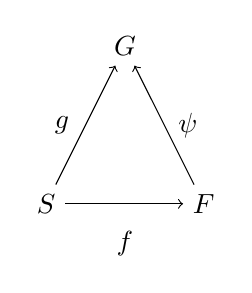
\begin{tikzpicture}
    \node(S) at (0, 0) {$S$};
    \node(F) at (2, 0) {$F$};
    \node(G) at (1, 2) {$G$};
    
    \draw [->] (S)--(F);
    \draw [->] (F)--(G);
    \draw [->] (S)--(G);
    
    \node at (1, -0.5) {$f$};
    \node at (1.8, 1) {$\psi$};
    \node at (0.2, 1) {$g$};
\end{tikzpicture}    
\end{center}

\subsection{Własności}

\subsection{Przykłady}